\begin{figure*}
\centering
\begin{subfigure}{.24\textwidth}
  \centering
  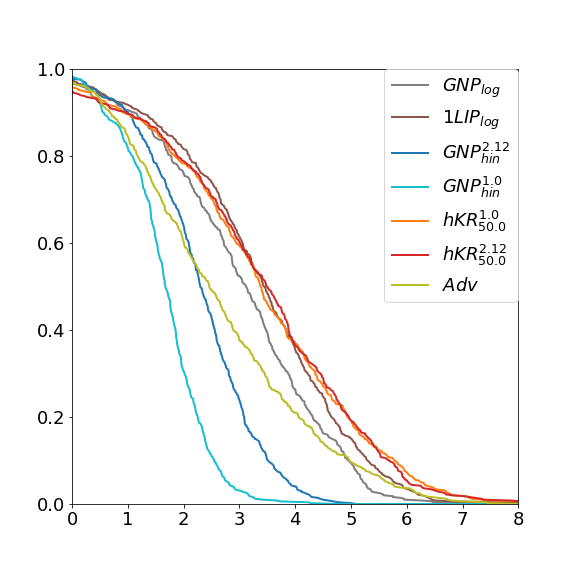
\includegraphics[width=1\linewidth]{cvpr_img/mnist_dense_adv_noise_norm_L2DeepFoolAttack.png}
  \caption{MNIST dense}
  \label{fig:l2norm_MLP_wass}
\end{subfigure}%
\begin{subfigure}{.24\textwidth}
  \centering
  
\includegraphics[width=1\linewidth]{cvpr_img/mnist_smallconfig_adv_noise_norm_L2DeepFoolAttack.png}
  \caption{MNIST CNN}
  \label{fig:l2_norm_VGG_wass}
\end{subfigure}
\begin{subfigure}{.24\textwidth}
  \centering
  
\includegraphics[width=1\linewidth]{cvpr_img/cifar10_verylarge_adv_noise_norm_L2DeepFoolAttack.png}
  \caption{CIFAR}
  \label{fig:l2_norm_MLP_lipsigmoid}
\end{subfigure}
\begin{subfigure}{.24\textwidth}
  \centering
  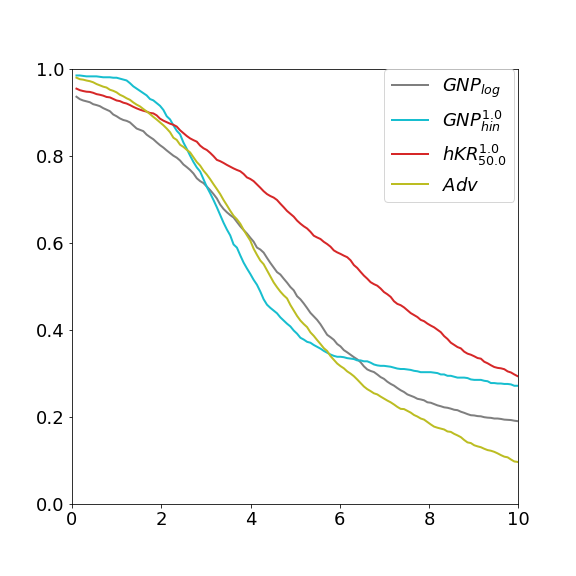
\includegraphics[width=1\linewidth]{cvpr_img/celeb_a_deepfool.png}
  \caption{CelebA}
  \label{fig:l2_norm_MLP_lipsigmoid}
\end{subfigure}
\caption{Accuracy (Y-axis) w.r.t. of $l_2$ norm of fooling noise with deepfool attack (X-axis) on 2000 images of the test set
}
\label{fig:deepfool_curves}
\end{figure*}

In the experiment, we compare five approaches: i) $Adv$ for Adversarial learning as in~\cite{Madry2017} , ii) $1LIP_{log}$ for log-entropy classifier with Björck orthonormalization and ReLU activation functions similar to Parseval networks~\cite{cisse_parseval_2017}, iii) $GNP^m_{hin}$ for gradient norm preserving classifiers based on hinge loss with margin $m$ as done in~\cite{li2019preventing} iv) $GNP_{log}$ for gradient norm preserving classifiers based on log entropy loss and v) $hKR^m_\alpha$ for gradient norm preserving classifiers based on the proposed hinge-KR with margin $m$ and coefficient $\alpha$. Note that, to the best of our knowledge, the $GNP_{log}$ hasn't been applied yet for adversarial defenses. To have a fair comparison, all the classifiers share the same dense or convolutional architectures except for the weight normalization and the activation functions. We set $\alpha$ to $50$ and margin $m$ to $1$ except for MNIST where we also consider $m=2.12$ to be comparable with the experiments in~\cite{li2019preventing}. For the $GNP$ classifiers, we apply Björck orthonormalization (15 steps with p=1) after the spectral normalization (this improves the convergence of the Björck algorithm). We use fullsort activation function for dense layers, and GroupSort2 for the convolutional ones.  Appendix~\ref{sec:networks_architecture} provides the full description of the architecture and the optimization process.

We consider three classification problems, two multi-class problems (MNIST~\cite{lecun-mnisthandwrittendigit-2010} and CIFAR-10~\cite{Krizhevsky09learningmultiple}) and a binary one (eyeglasses detection in Celeba-A dataset \cite{liu2015faceattributes}). For MNIST and CIFAR-10, we use standard configurations with 10 classes and no data augmentation, $50 000$ examples in the training set and $10 000$ examples in the test set. In the binary problem, we consider the separation between people with or without eyeglasses on the CelebA dataset with 128x128x3 centered images. This is an unbalanced classification problem with $16914$ examples in the training set ($38\%$ with eyeglasses) and $16914$ examples in the test set ($38\%$ with eyeglasses).

Figure \ref{fig:deepfool_curves} presents the robustness against $l_2$ attacks with \textit{DeepFool} attack~\cite{moosavi-deepfool15} on the different datasets. We use this type of attack since none of the tested approaches is specifically built to resist to it. We can observe that the $hKR^m_\alpha$ approach is at the top of robustness on all the dataset and systematically better than $GNP_{log}$ on all datasets and $GNP^m_{hin}$ on the multiclass problem for the same value of $m$. On the CelebA dataset, $GNP^m_{hin}$ and the adversarial approach $Adv$ start with a better accuracy, but don't resist to large attacks. $GNP_{log}$ and $1LIP$ have good performances on MNIST and CIFAR but their performances decrease when the models are deeper as for CelebA dataset ($1LIP$ was unable to converge on CelebA). To compare the different defense methods, we also apply a combination of the state-of-the art attacks $FGSM$~\cite{Goodfellow2014a}, $PGD$~($l_2PGD$) \cite{Madry2017} and  Carlini and Wagner ($l_2CW$) \cite{carlini2017towards} on 500 images of the test set. All attacks are performed with the  foolbox library~\cite{rauber2017foolbox}. For each value of $\epsilon$, we run all the attacks and consider it as a success if at least one of them has succeeded. The results are presented in Figure~\ref{fig:combine_curves} and Table~\ref{tab:celeba_comparison} details the robustness values for CelebA. The results confirm and amplify the ones obtained with deepfool attacks. $hKR^m_\alpha$ obtain the highest level of robustness in all the situations for low and high values of $\epsilon$. 
$Adv$ has the highest robustness w.r.t. $FGSM$ attacks, since it was designed against to, but is a bit less resistant w.r.t. $l_2PGD$ and weak w.r.t. $l_2CW$. $hKR^m_\alpha$ is especially strong w.r.t. Carlini and Wagner attack even with high values of $\epsilon$. The discrepancy between the robustness of the approaches increase when models become deeper. On the CelebA dataset,  $GNP_{log}$ have difficulties to resist to higher noise. As expected, $hKR^m_\alpha$ seems to take most advantage of the gradient norm preserving architecture and obtains robustness against large attacks with an acceptable decrease of accuracy without noise. 

Moreover, Table \ref{tab:celeba_comparison} shows that, for the proposed solution, accuracies w.r.t. $\epsilon$ are similar regardless the attacks. This suggests that optimal attacks are the same, and they are in the direction of the gradient of the classifier. This confirms the intuition pointed out in section~\ref{sec:khr_properties} that optimal attack consists on traveling along the optimal transport map. In Figure~\ref{fig:Deep_fool_CelebA}, we compare adversarial images obtained with $l_2$ deepfool for the different models. The first row corresponds to the initial image. The following rows except the last one, are pictures obtained after attacks for the different models. We design the attacks to push the image just beyond the classification boundary (50/50).  For the Madry et al. approach ($Adv$) the noise is barely detectable. The noise is more visible with the gradient preserving approaches $GNP_{log}$ and $GNP^m_{hin}$ but it is still hard to interpret and sometimes meaningless. In contrast to the other approaches, the noise required to change the output class for the $hKR$ classifier is highly structured, and interpretable. For people without glasses, the attack adds noise around the eyes and at the top of the nose. For people with eyeglasses, the attack tends to erase the glasses around the eyes and at the top of the nose. 

The last row corresponds to the scheme proposed in Section~\ref{sec:khr_properties} $att(\hat{f},\textbf{x})\approx x-2*\hat{f}(\textbf{x})*\nabla_x \hat{f}(\textbf{x})$ where $\hat{f}$ is the $hKR^1_{50}$ model. Indeed, if $\nabla_x \hat{f}(\textbf{x})=1$ and $\hat{f}(\textbf{x})$ is the distance between the $\textbf{x}$ and its image with respect to the transport, we expect to have $att(\hat{f},\textbf{x})=tr(\hat{f},\textbf{x})$. The  shifts are similar to the attacks and even more meaningful. This confirms that attacks against $hKR$ can be interpreted as a transportation from a class to the other one and then requires to explicitly change the transport image in the opposite class. This suggests that attacks can explain classification for the $hKR$ model. Moreover, the gradient of this model allows to build this explanation without relying on time-consuming algorithms.  



\begin{figure*}
\centering
\begin{subfigure}{.24\textwidth}
  \centering
  
\includegraphics[width=1\linewidth]{cvpr_img/mnist_dense__minAccuracy_L2attacks.png}
  \caption{MNIST dense}
\end{subfigure}%
\begin{subfigure}{.24\textwidth}
  \centering
  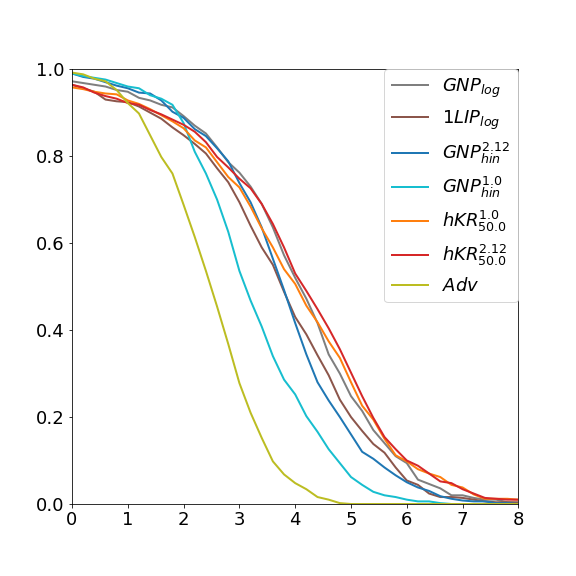
\includegraphics[width=1\linewidth]{cvpr_img/mnist_smallconfig__minAccuracy_L2attacks.png}
  \caption{MNIST CNN}
\end{subfigure}
\begin{subfigure}{.24\textwidth}
  \centering
  
\includegraphics[width=1\linewidth]{cvpr_img/cifar10_verylarge__minAccuracy_L2attacks.png}
  \caption{CIFAR}
\end{subfigure}
\begin{subfigure}{.24\textwidth}
  \centering
  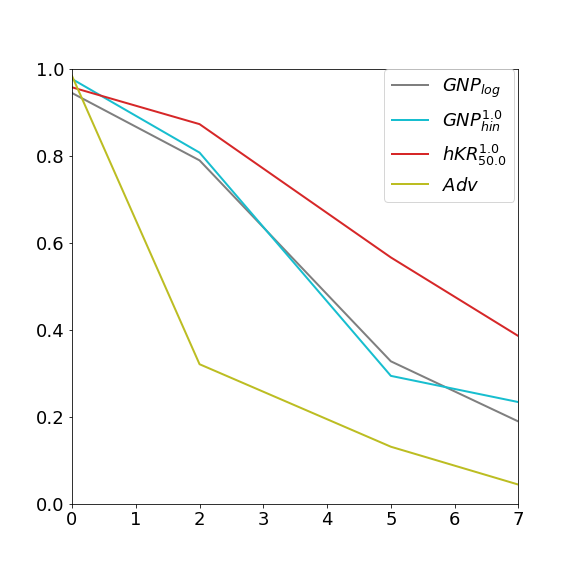
\includegraphics[width=1\linewidth]{cvpr_img/celeb_a_deepfool_all.png}
  \caption{CelebA}
\end{subfigure}
\caption{Accuracy (Y-axis) w.r.t. of $l_2$ norm of $FGSM$, $l_2PGD$, deepfool and $l_2$ Carlini and Wagner combined attacks on 500 images of the test set
}
\label{fig:combine_curves}
\end{figure*}



\begin{table}[]
    \centering

\begin{tabular}{|c|c|c|c|c|c|}
\hline
                          & $\epsilon$   & $Adv$ & $GNP_{hin}$ & $GNP_{log}$ & $hKR_{50}$\\ \hline
Base                      &   0   &   \textbf{98.04 }  &  97.2        &       94.51    &     96.07         \\ \hline
\multirow{2}{*}{$FGSM$} & $2$     &    \textbf{90.52 } &   86.79      &         81.40  &    87.44             \\ \cline{2-6} 
                          &  $5$  &  \textbf{ 82.96  } &     37.70    &      43.90     &     64.01                \\ \hline
\multirow{2}{*}{$l_2 GPD$}&  $2$            & 81.98    &     88.65    &    84.17       &\textbf{88.75  }           \\ \cline{2-6} 
                          &    $5$      &   61.35      &    34.90     &    48.02       &              \textbf{69.79  }     \\ \hline
\multirow{2}{*}{$l_2 CW$} &  $2$            & 32.14    &   80.80      &    79.02       &        \textbf{ 88.62 }         \\ \cline{2-6} 
                          &      $5$          &  13.17  &    29.46   &   32.81         &      \textbf{56.44     }    \\ \hline
\end{tabular}
    \caption{Robustness w.r.t. various attacks on CelebA dataset}
    \label{tab:celeba_comparison}
\end{table}


\begin{figure*}
\centering

    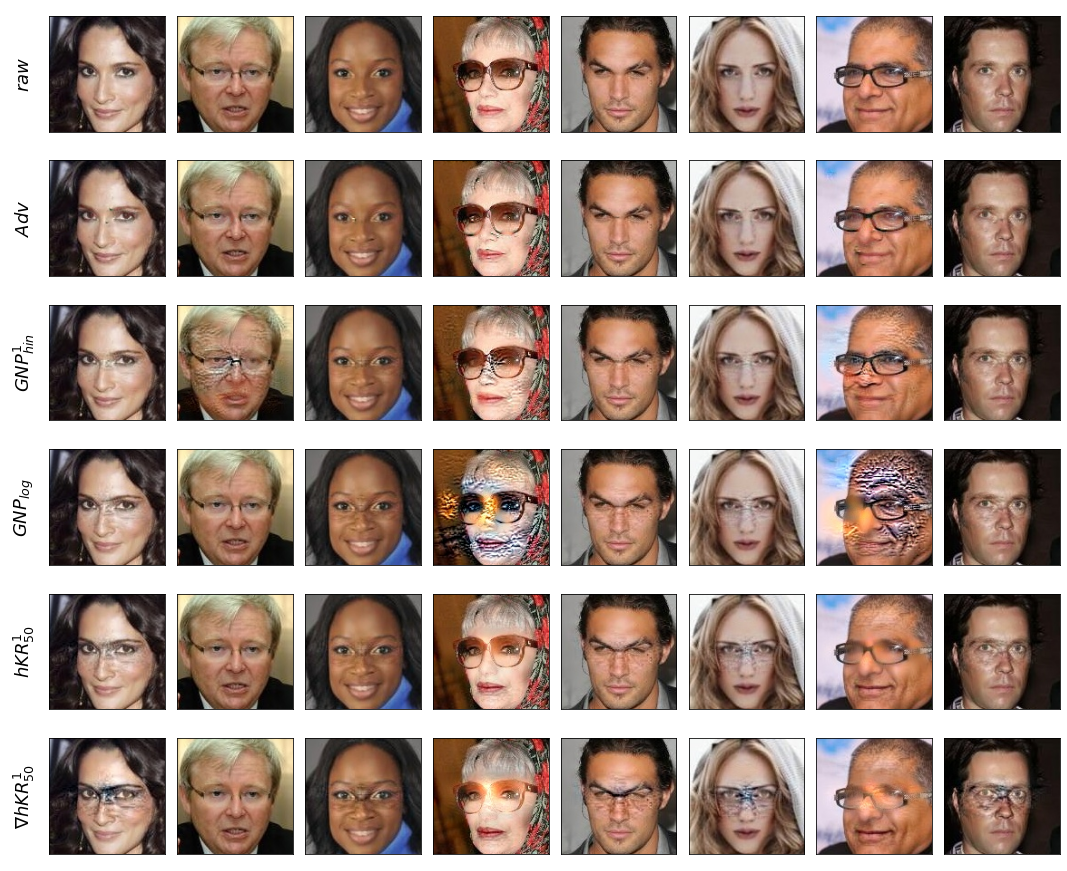
\includegraphics[width=1\linewidth]{cvpr_img/adversaries.png}

\caption{Adversarial examples on CelebA dataset. The first row is the input image.}
%Classical networks (1st line) and 1-lipschitz networks learned with binary crossentropy (2nd line) lead to invisble noise, whereas proposed solution (3rd line) add or remove dark pixels around the nasolabial fold}
\label{fig:Deep_fool_CelebA}
\end{figure*}
